\documentclass[12pt]{article}
\usepackage[utf8]{inputenc}
%\usepackage[sectionbib]{natbib}
\usepackage[margin=1in]{geometry}
%\usepackage{mathrsfs}
\usepackage{multirow,multicol}
\usepackage{amsfonts}
\usepackage{amsmath,amssymb,amsthm}
\usepackage[mathscr]{euscript}
\usepackage{comment}
\usepackage{graphicx,color}
\graphicspath{{image/}}
\usepackage{mathtools}
\usepackage{mathabx} %widecheck
\usepackage[linesnumbered,ruled,vlined]{algorithm2e}
\usepackage{setspace}
\usepackage{sectsty}
\usepackage{makecell}
\usepackage{chngcntr}
\usepackage{apptools}
\usepackage{caption}
\usepackage{subcaption}
\usepackage{booktabs}
\usepackage{etoolbox}
\usepackage{bbm}

\usepackage{tabularx}
\newcolumntype{Y}{>{\raggedleft\arraybackslash}X}
\newcolumntype{Z}{>{\centering\arraybackslash}X}
\usepackage{enumitem}
\usepackage{underscore} 
\usepackage{array} 
\usepackage{arydshln}
\usepackage{soul}
\usepackage{tikz}
\usetikzlibrary{matrix}
% \usepackage{subfig}
\usepackage[english]{babel}
%\usepackage[toc,page]{appendix}
\usepackage[colorlinks=true,linkcolor=blue,urlcolor=black,citecolor=blue,bookmarksopen=true]{hyperref}
\usepackage{bookmark}
\usepackage{multirow} % use multirow
\let\counterwithout\relax
\let\counterwithin\relax
\usepackage{lipsum}
%\newenvironment{bottompar}{\par\vspace*{\fill}}{\clearpage} %for bottompar
\usepackage{calrsfs} % for calligraphic letters in the OMS encoding 

%\usepackage{siunitx} % use S[table-format=2.2] in tables to align decimal points

\DeclareMathAlphabet{\pazocal}{OMS}{zplm}{m}{n} % usepackage calrsfs

\DeclareFontFamily{OT1}{pzc}{}
\DeclareFontShape{OT1}{pzc}{m}{it}{<-> s * [1.10] pzcmi7t}{}
\DeclareMathAlphabet{\mathpzc}{OT1}{pzc}{m}{it}

\usepackage{natbib}
\bibliographystyle{apalike}

%\usepackage{xr}
%\externaldocument{Supplement}

\newtheorem{assumption}{Assumption}
\newtheorem{condition}{Condition}
\newtheorem{example}{Example}
\newtheorem{definition}{Definition}
\newtheorem{lemma}{Lemma}
\newtheorem{proposition}{Proposition}
\newtheorem{theorem}{Theorem}
\newtheorem{corollary}{Corollary}
\newtheorem{innercustom}{Lemma}
%\theoremstyle{remark}
\newtheorem{remark}{Remark}
\usepackage{epstopdf}
\newenvironment{custom}[1]
{\renewcommand\theinnercustom{#1}\innercustom}
{\endinnercustom}

\newcommand{\algcomment}[1]{%
	\vspace{-\baselineskip}%
	\noindent%
	{\footnotesize #1\par}%
	\vspace{\baselineskip}%
}
\newcolumntype{P}[1]{>{\centering\arraybackslash}p{#1}}
\newcommand{\norm}[1]{\left\lVert#1\right\rVert}
\newcommand{\ts}{\textsuperscript}
\newcommand{\bm}{\boldsymbol}
\newcommand{\cm}[1]{\mbox{\boldmath$\mathscr{#1}$}}
\newcommand{\cmt}[1]{\mbox{\boldmath\scriptsize$\mathscr{#1}$}}
\newcommand{\cmtt}[1]{\mbox{\boldmath\tiny$\mathscr{#1}$}}
\newcommand{\Fr}{{\mathrm{F}}}
\newcommand{\op}{{\mathrm{op}}}
\newcommand{\est}{{\mathrm{est}}}
\newcommand{\pred}{{\mathrm{pred}}}
\newcommand{\ma}{{\mathrm{MA}}}
\newcommand{\ar}{{\mathrm{AR}}}
\newcommand{\rowsp}{\mathrm{rowsp}}
\newcommand{\colsp}{\mathrm{colsp}}
\newcommand{\rsc}{{\mathrm{rsc}}}
\newcommand{\dev}{{\mathrm{dev}}}
\newcommand{\init}{{\mathrm{init}}}

\newcommand{\card}{{\mathrm{card}}}
\newcommand{\HW}{{\mathrm{HW}}}
\newcommand{\stcomp}[1]{{#1}^\complement} % set complement
\def\HH{{\mathrm{\scriptscriptstyle\mathsf{H}}}}


%%%%%%%%%%%%%%%%%%%%%%%%%%%%%%%%%%%%%%%%%%%

%\mathtoolsset{showonlyrefs}
\DeclareMathOperator*{\vect}{vec}
\DeclareMathOperator*{\rank}{rank}
\DeclareMathOperator*{\trace}{tr}
\DeclareMathOperator*{\argmin}{arg\,min}
\DeclareMathOperator*{\argmax}{arg\,max}
\DeclareMathOperator*{\sgn}{sgn}
\DeclareMathOperator*{\diag}{diag}
\DeclareMathOperator*{\cov}{cov}
\DeclareMathOperator*{\var}{var}
\DeclareMathOperator*{\stk}{stack}
\DeclarePairedDelimiter\floor{\lfloor}{\rfloor}
%%%%%%%%%%%%%%%%%%%%%%%%%%%%%%%%%%%%%%%%%%%%%
\newcommand{\red}[1]{\textcolor{red}{#1}}
\newcommand{\blue}[1]{\textcolor{blue}{#1}}
\newcommand{\ZY}[1]{\textcolor{magenta}{(ZY: #1)}}
%%%%%%%%%%%%%%%%%%%%%%%%%%%%%%%%%%%%%%%%%%%%%
\baselineskip=15.5pt
\renewcommand{\arraystretch}{1}
\renewcommand{\baselinestretch}{1.5}
\renewcommand\tabcolsep{3pt}
\numberwithin{equation}{section}


\title{\vspace{-20pt} Tensor-valued Time Series Factor Model}

\begin{document}
	
\section{Model}
Target Tensor $\cm{Y}\in\mathbb{R}^{T\times K\times N_Y}$. Observed $\bm{Y}\in\mathbb{R}^{T\times N_Y}$.

Auxiliary tensor $\cm{X}\in\mathbb{R}^{T\times K\times N_X}$ is fully observed.

Suppose
\begin{gather}
	\bm{Y}=\sum_{i=1}^r\bm{g}_i\circ\bm{\Lambda}_i^Y\\
	\cm{X}=\sum_{i=1}^r\bm{g}_i\circ\bm{w}_i\circ\bm{\Lambda}_i^X
\end{gather}

\section{Estimation}
Consider loss function
\begin{gather}
	\Big\lVert\cm{X}-\sum_{i=1}^r\bm{g}_i\circ\bm{w}_i\circ\bm{\Lambda}_i^X \Big\rVert_F+\gamma\Big\lVert\bm{Y}-\sum_{i=1}^r\bm{g}_i\circ\bm{\Lambda}_i^Y\Big\rVert_F\\
	\Big\lVert\cm{X}_{(1)}-\sum_{i=1}^r\bm{g}_i\circ(\bm{\Lambda}_i^X\otimes\bm{w}_i)\Big\rVert_F+\gamma\Big\lVert\bm{Y}-\sum_{i=1}^r\bm{g}_i\circ\bm{\Lambda}_i^Y\Big\rVert_F
\end{gather}
Let $\bm{H}_i = \bm{\Lambda}_i^X\otimes\bm{w}_i$, $\bm{\Lambda}_{(\gamma)}^T=(\bm{\Lambda}_Y^T, \bm{H}^T)$. Identification condition $\frac{1}{N_Y+KN_X}\bm{\Lambda}_{(\gamma)T}\bm{\Lambda}_{(\gamma)}=\bm{I}_r$. 

Estimate $\bm{\Lambda}^X$ and $\bm{W}$ with $\sum_{i=1}^r\lVert\bm{H}_i-\bm{\Lambda}_i^X\otimes\bm{w}_i\rVert_F$. Fold $\bm{H}_i$ to $\bm{H}_i^M\in\mathbb{R}^{N_Y\times K}$, then the problem becomes $\sum_{i=1}^r\lVert\bm{H}_i^M-\bm{\Lambda}_i^X\circ\bm{w}_i\rVert_F$. Assume $\bm{H}_i^{M*}=\bm{\Lambda}_i^{X*}\circ\bm{w}_i^*$, then $\bm{H}_i^{M*}$ becomes a rank-one matrix. The identification condition of $\bm{\Lambda}_i^{X*}$ and $\bm{w}_i^*$ is $\lVert\bm{\Lambda}_i^{X*}\rVert=1$, since the SVD of $\bm{H}_i^{M*}$ is unique, and $\bm{\Lambda}_i^{X*}$ is equivalent to the singular factor of $\bm{H}_i^{M*}$. 

\section{Algorithm}
\begin{enumerate}
	\item Combine $\cm{X}_{(1)}$ and $\bm{Y}$
	\item Estimate $\widehat{\bm{\Lambda}}_{(\gamma)}$ by PCA.
	\item Estimate $\widehat{\bm{G}}$ by weighted regression.
	\item Estimate $\bm{\Lambda}_{i}^X$ and $\bm{W}_i$ for each $\bm{H}_i$ by rank-1 SVD.
	\item Orthogonalize $\bm{\Lambda}^X$ with SVD. Multiply the same orthogonalization matrix to $\bm{W}$ 
\end{enumerate}

\section{Simulation}
We set $N_X=N_Y=K\in\{5,10,15,20,25\}$ and $r\in\{2,3,4\}$. 
\begin{figure}[hbt]
  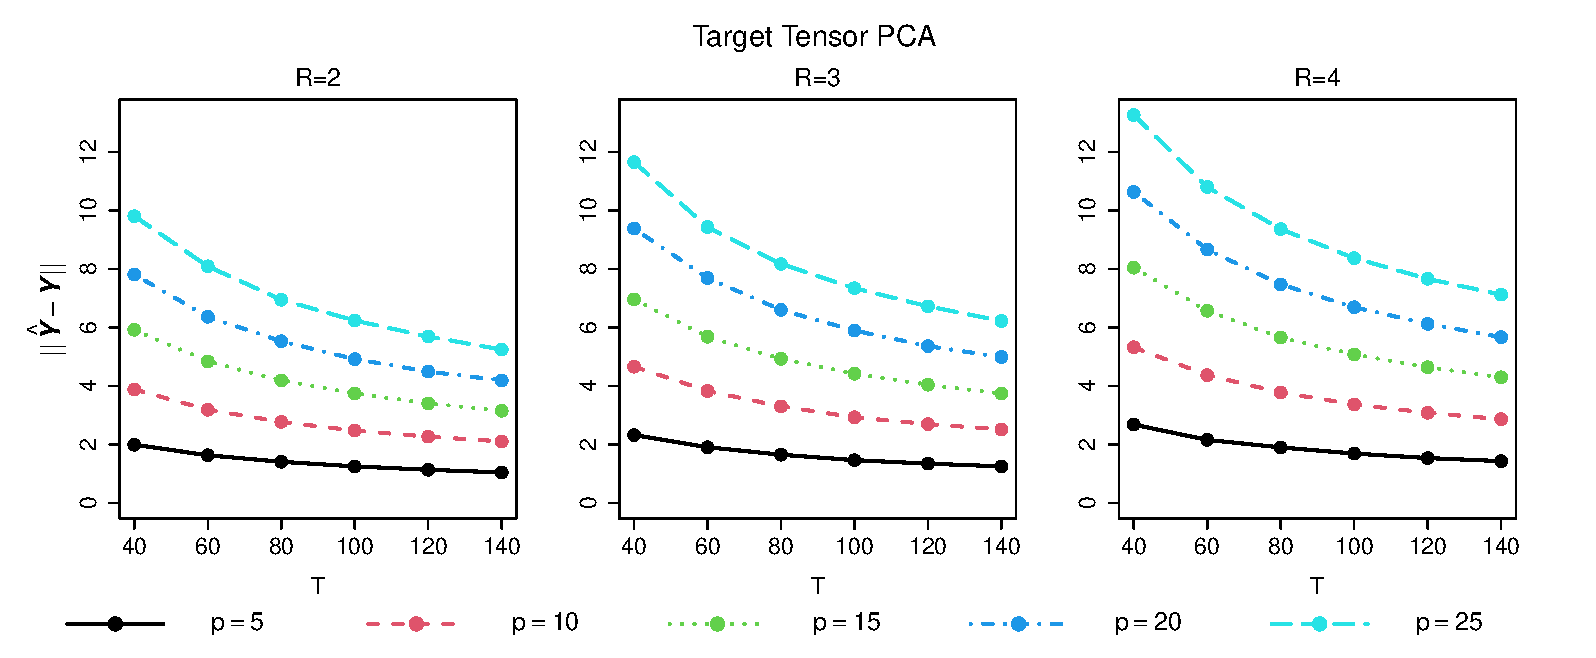
\includegraphics[width=\textwidth]{plot1.eps}
\end{figure}



\section{FRED-Q}
This data set contains low-frequency quarterly data from FRED-QD, which records 179 indexes classified by NIPA, Industrial Production, Employment \& Unemployment, Housing, Prices, Interest Rates, Money \& Credit, and others; high-frequency quarterly data from FRED-MD, which records 112 indexes classified by Output \& Income, Trade, Labor Market, Housing, Money \& Credit, Interest \& Exchange Rates and Prices. We take the data from 1975 to 1995, in total of 20 years.

We take $r=5$, $\gamma = 1.8$. The estimation to the missed GDP in FRED-Q is given as below.
\begin{figure}[hbt]
  \centering
  \includegraphics[width=0.9\textwidth]{TTPCAr5.png}
\end{figure}







\end{document}
